\chapter{Mecânica quântica para químicos: sistemas-modelo}\label{ch:b3:quantum-model-systems}

Três pequenos frascos estão sobre a bancada, cada um com uma solução de um
corante de cianina em etanol: o primeiro é magenta, o segundo azul, o
terceiro de um azul-esverdeado profundo que absorve no vermelho distante.
As três moléculas são construídas do mesmo modo --- dois anéis nitrogenados
idênticos ligados por uma cadeia de átomos de carbono --- e diferem apenas
no comprimento dessa cadeia, de dois em dois átomos de carbono. Alongue a
cadeia e a cor se desloca para o vermelho. Em 1949, um químico explicou a
série com um dos problemas mais simples da mecânica quântica: um elétron
livre para se mover ao longo de um segmento de comprimento fixo, uma
``\omterm{def:b3:quantum-model-systems:box}{partícula na caixa}''. Este capítulo monta a maquinaria por trás dessa
explicação --- \omterm{def:b3:quantum-model-systems:operator}{operadores}, \omterm{def:b3:quantum-model-systems:operator}{autovalores}, a \omterm{thm:b3:quantum-model-systems:schrodinger}{equação de Schrödinger} --- e
resolve os sistemas-modelo que a química usa todos os dias: a caixa, o
\omterm{def:b3:quantum-model-systems:oscillator}{oscilador harmônico} de uma ligação que vibra, o \omterm{def:b3:quantum-model-systems:rotor}{rotor rígido} de uma
molécula que gira, o átomo de hidrogênio e a barreira que uma partícula
leve consegue atravessar sem ter energia para escalá-la.

\begin{recall}
O volume do 1.º ano mostrou que a energia de um átomo é quantizada (níveis
de energia, estados fundamental e excitados, as raias do hidrogênio) e que
um fóton transporta $E = h\nu = hc/\lambda$. O volume do 2.º ano descreveu
um elétron por uma função de onda $\psi$ cujo quadrado é uma densidade de
probabilidade, separou os orbitais do hidrogênio em partes radial e angular
e contou seus nós; ele tomou as funções de onda do hidrogênio como dadas.
Elas são deduzidas aqui, na seção 5. Da física: o momento linear $p = mv$ e
o comprimento de onda de de Broglie $\lambda = h/p$.
\end{recall}

\begin{omfigure}
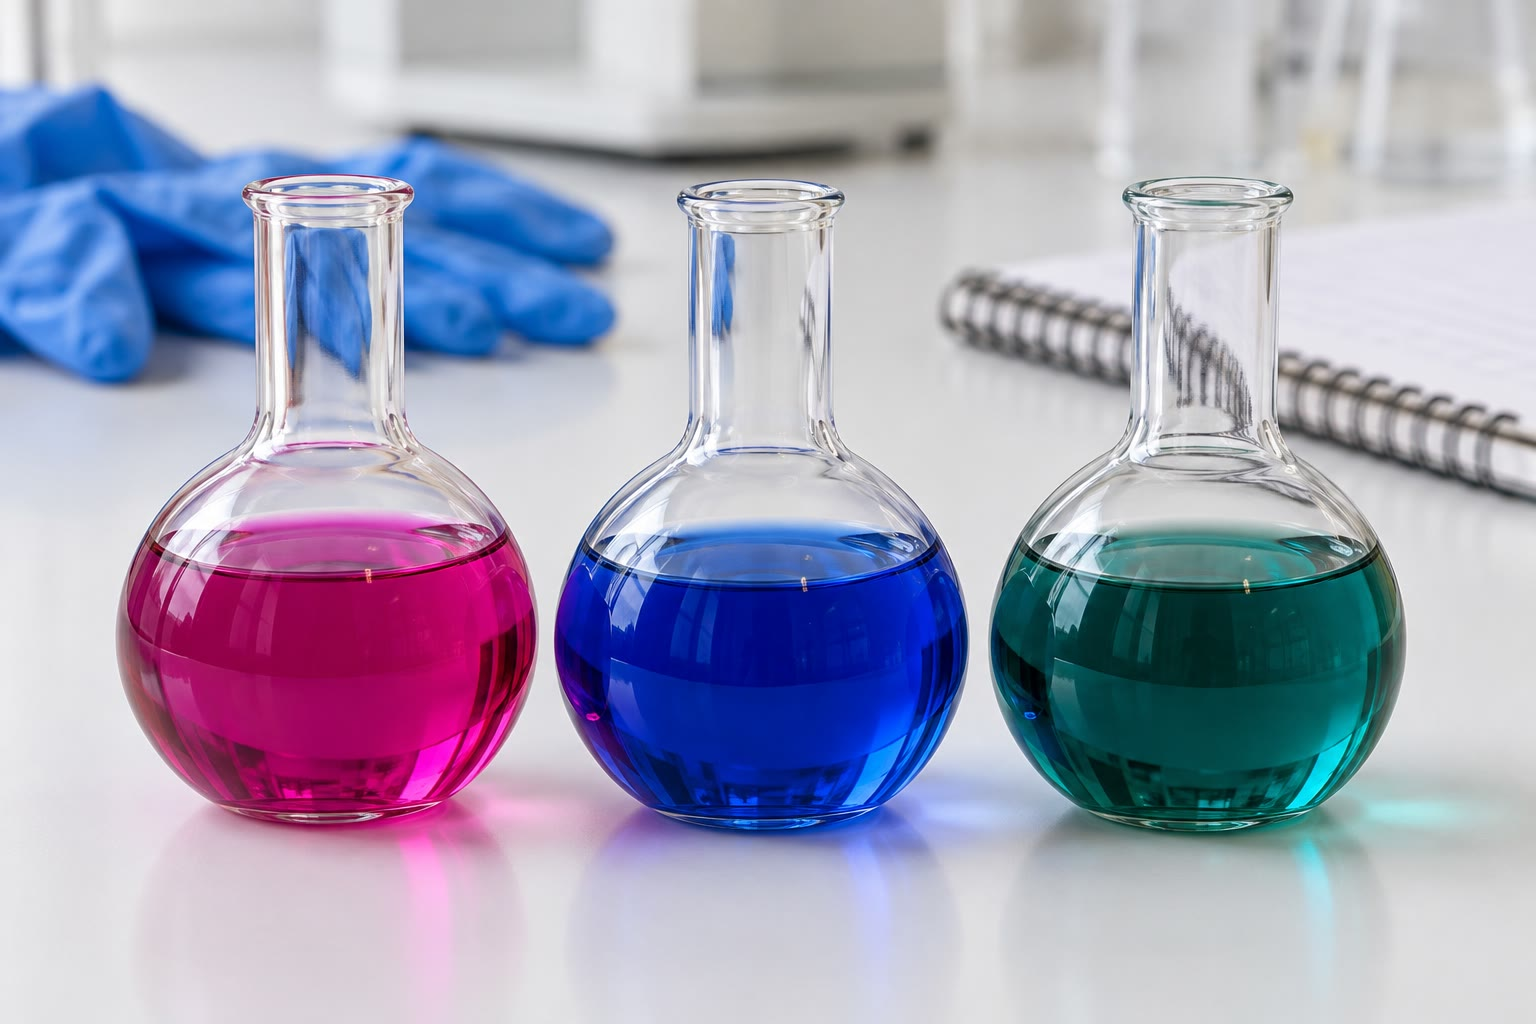
\includegraphics[width=0.62\linewidth]{images/book4/ai/b3-01-dyes.jpg}

{\small Soluções de três corantes de cianina de uma mesma família. Cada par
de átomos de carbono acrescentado à cadeia desloca a absorção para o vermelho.}
\end{omfigure}

\section{Operadores, autovalores e a equação de Schrödinger}

A mecânica clássica atribui a uma partícula uma posição e um momento linear
a cada instante. A mecânica quântica atribui-lhe um estado, a função de onda
$\psi$, e substitui cada grandeza mensurável por uma operação efetuada sobre $\psi$.

\begin{definition}[Operador, autofunção, autovalor]\label{def:b3:quantum-model-systems:operator}
Um \emph{operador}\index{operador} $\hat A$ é uma regra que transforma uma
função em outra função: $\hat A f = g$. Ele é linear se $\hat A(\lambda f +
\mu g) = \lambda\hat Af + \mu\hat Ag$. Uma função não nula $f$ tal que
$\hat Af = a f$ para um número $a$ é uma \emph{autofunção}\index{autofuncao@autofunção}
de $\hat A$, e $a$ é o \emph{autovalor}\index{autovalor} correspondente.
\end{definition}

\begin{example}[Os operadores de posição e de momento linear]\label{ex:b3:quantum-model-systems:xp}
Em uma dimensão, o \omterm{def:b3:quantum-model-systems:operator}{operador} posição multiplica por $x$, $\hat x f = xf$,
e o \omterm{def:b3:quantum-model-systems:operator}{operador} momento linear deriva, $\hat p f = -\iu\hbar\,
\dd f/\dd x$, com $\hbar = h/2\pi$. A função $\eu^{\iu kx}$ é uma
\omterm{def:b3:quantum-model-systems:operator}{autofunção} de $\hat p$ com \omterm{def:b3:quantum-model-systems:operator}{autovalor} $\hbar k$: uma onda de comprimento de
onda $\lambda = 2\pi/k$ tem momento linear $h/\lambda$, a relação de de Broglie.
A função $\sin kx$ não é \omterm{def:b3:quantum-model-systems:operator}{autofunção} de $\hat p$ (sua derivada é um
cosseno), mas é \omterm{def:b3:quantum-model-systems:operator}{autofunção} de $\hat p^2 = -\hbar^2\,\dd^2/\dd x^2$, com
\omterm{def:b3:quantum-model-systems:operator}{autovalor} $\hbar^2k^2$.
\end{example}

\begin{definition}[Operador hermitiano, valor esperado]\label{def:b3:quantum-model-systems:hermitian}
Escreva $\langle f|g\rangle = \int f^*g\,\dd\tau$ para duas funções que se
anulam nas fronteiras da região. Um \omterm{def:b3:quantum-model-systems:operator}{operador} é \emph{hermitiano}\index{operador hermitiano}
se $\langle f|\hat Ag\rangle = \langle \hat Af|g\rangle$ para todas essas
$f$ e $g$. Para um estado normalizado $\psi$ ($\langle\psi|\psi\rangle = 1$), o
\emph{valor esperado}\index{valor esperado} de $\hat A$ é
$\langle A\rangle = \langle\psi|\hat A\psi\rangle$: a média de muitas
medidas feitas sobre sistemas preparados de modo idêntico.
\end{definition}

As regras de trabalho da química quântica --- seus postulados --- podem
agora ser enunciadas de uma só vez: toda grandeza mensurável é representada
por um \omterm{def:b3:quantum-model-systems:hermitian}{operador hermitiano}; uma medida dá um de seus \omterm{def:b3:quantum-model-systems:operator}{autovalores}; e, se
$\psi$ é uma \omterm{def:b3:quantum-model-systems:operator}{autofunção} de $\hat A$, toda medida sobre ela dá o mesmo valor,
seu \omterm{def:b3:quantum-model-systems:operator}{autovalor}.

\begin{theorem}[Operadores hermitianos]\label{thm:b3:quantum-model-systems:hermitian-real}
Os \omterm{def:b3:quantum-model-systems:operator}{autovalores} de um \omterm{def:b3:quantum-model-systems:hermitian}{operador hermitiano} são reais. Duas \omterm{def:b3:quantum-model-systems:operator}{autofunções} com
\omterm{def:b3:quantum-model-systems:operator}{autovalores} diferentes são ortogonais: $\langle f_1|f_2\rangle = 0$.
\end{theorem}

\begin{proof}
Seja $\hat Af = af$. Então $\langle f|\hat Af\rangle = a\langle f|f\rangle$ e
$\langle\hat Af|f\rangle = a^*\langle f|f\rangle$. O \omterm{def:b3:quantum-model-systems:operator}{operador} é \omterm{def:b3:quantum-model-systems:hermitian}{hermitiano},
logo as duas são iguais, e $\langle f|f\rangle > 0$: $a = a^*$. Sejam agora $\hat Af_1
= a_1f_1$ e $\hat Af_2 = a_2f_2$ com $a_1 \ne a_2$, ambos reais. Então
$\langle f_1|\hat Af_2\rangle = a_2\langle f_1|f_2\rangle$ e $\langle\hat Af_1|
f_2\rangle = a_1\langle f_1|f_2\rangle$; sua igualdade dá $(a_2 - a_1)
\langle f_1|f_2\rangle = 0$, logo $\langle f_1|f_2\rangle = 0$.
\end{proof}

Um valor medido é um número real, e é por isso que os observáveis devem ser
\omterm{def:b3:quantum-model-systems:hermitian}{hermitianos}; a ortogonalidade é o que faz dos orbitais de um átomo, ou dos
níveis de uma caixa, um conjunto limpo de estados independentes.

\begin{definition}[Comutador]\label{def:b3:quantum-model-systems:commutator}
O \emph{comutador}\index{comutador} de dois \omterm{def:b3:quantum-model-systems:operator}{operadores} é $[\hat A,\hat B] =
\hat A\hat B - \hat B\hat A$. Os \omterm{def:b3:quantum-model-systems:operator}{operadores} comutam se seu comutador é
nulo.
\end{definition}

\begin{example}[O comutador canônico]\label{ex:b3:quantum-model-systems:canonical}
Para toda função $f$, $\hat x\hat pf = -\iu\hbar xf'$ e $\hat p\hat xf =
-\iu\hbar(f + xf')$. A diferença é $[\hat x,\hat p]f = \iu\hbar f$, logo
$[\hat x,\hat p] = \iu\hbar$: posição e momento linear não comutam. Essa
única relação está na base do princípio da incerteza e, mais adiante, de
todo o espectro do \omterm{def:b3:quantum-model-systems:oscillator}{oscilador harmônico}.
\end{example}

\begin{proposition}[Operadores que comutam]\label{prop:b3:quantum-model-systems:commuting}
Se $\hat A$ e $\hat B$ comutam e $f$ é uma \omterm{def:b3:quantum-model-systems:operator}{autofunção} de $\hat A$
com um \omterm{def:b3:quantum-model-systems:operator}{autovalor} não degenerado $a$, então $f$ também é \omterm{def:b3:quantum-model-systems:operator}{autofunção} de
$\hat B$.
\end{proposition}

\begin{proof}
$\hat A(\hat Bf) = \hat B\hat Af = a(\hat Bf)$: a função $\hat Bf$ é uma
\omterm{def:b3:quantum-model-systems:operator}{autofunção} de $\hat A$ com o mesmo \omterm{def:b3:quantum-model-systems:operator}{autovalor} $a$, ou é nula. Como o
\omterm{def:b3:quantum-model-systems:operator}{autovalor} é não degenerado, $\hat Bf$ é um múltiplo de $f$, digamos $bf$.
\end{proof}

O \omterm{def:b3:quantum-model-systems:operator}{operador} da energia é o hamiltoniano. Para uma partícula de massa $m$ em
um potencial $V$, a energia clássica $p^2/2m + V$ torna-se um \omterm{def:b3:quantum-model-systems:operator}{operador}.

\begin{definition}[Operador hamiltoniano]\label{def:b3:quantum-model-systems:schrodinger}
O \emph{operador hamiltoniano}\index{operador hamiltoniano} de uma partícula de
massa $m$ que se move em um potencial $V(\mathbf r)$ é
\[
\hat H = -\frac{\hbar^2}{2m}\nabla^2 + V(\mathbf r), \qquad \nabla^2 =
\frac{\partial^2}{\partial x^2} + \frac{\partial^2}{\partial y^2} +
\frac{\partial^2}{\partial z^2},
\]
e, para várias partículas, a soma de seus termos cinéticos e de todas as
suas energias potenciais.
\end{definition}

\begin{theorem}[A equação de Schrödinger]\label{thm:b3:quantum-model-systems:schrodinger}
Os estados de energia definida de um sistema --- seus estados estacionários ---
são as \omterm{def:b3:quantum-model-systems:operator}{autofunções} de seu hamiltoniano, e suas energias permitidas são os
\omterm{def:b3:quantum-model-systems:operator}{autovalores}:
\[
\hat H\psi = E\psi,
\]
a \emph{equação de Schrödinger}\index{equacao de Schrodinger@equação de Schrödinger} independente do tempo.
Uma $\psi$ aceitável é unívoca, contínua e de quadrado integrável
(pode ser normalizada).
\end{theorem}
\begin{proof}[Estatuto]
Trata-se de um postulado, justificado por suas consequências: os níveis de
todos os sistemas resolvidos a seguir concordam com a espectroscopia. A
equação dependente do tempo, da qual esta é o caso estacionário, pertence à física.
\end{proof}

São as condições de contorno que quantizam: uma equação diferencial tem
soluções para todo $E$, mas só um conjunto discreto delas permanece finito
e contínuo. A química torna-se então uma questão de escolher um potencial,
resolver e ler os \omterm{def:b3:quantum-model-systems:operator}{autovalores}.

\begin{method}[Resolver um modelo unidimensional]\label{met:b3:quantum-model-systems:one-dimensional}
\begin{enumerate}
  \item Escreva o potencial $V(x)$ e o hamiltoniano; divida o espaço em
        regiões onde $V$ é simples.
  \item Resolva $-\frac{\hbar^2}{2m}\psi'' + V\psi = E\psi$ em cada região: senos
        e cossenos onde $E > V$, exponenciais reais onde $E < V$.
  \item Imponha as condições: $\psi = 0$ onde $V$ é infinito; $\psi$
        e $\psi'$ contínuas em um degrau finito; $\psi \to 0$ no infinito.
  \item As condições só são satisfeitas para certos $E$: esses são os níveis.
  \item Normalize cada \omterm{def:b3:quantum-model-systems:operator}{autofunção}; conte seus nós como verificação (o
        $n$-ésimo nível de um problema unidimensional tem $n - 1$ nós).
\end{enumerate}
\end{method}

\section{A partícula na caixa}

\begin{definition}[Partícula na caixa, modelo do elétron livre]\label{def:b3:quantum-model-systems:box}
Uma \emph{partícula na caixa}\index{particula na caixa@partícula na caixa} move-se livremente ($V = 0$)
entre $x = 0$ e $x = L$ e não pode sair ($V = \infty$ fora). O
\emph{modelo do elétron livre}\index{modelo do eletron livre@modelo do elétron livre} de uma molécula
conjugada trata seus elétrons $\pi$ como partículas independentes em uma
caixa cujo comprimento é o da cadeia conjugada.
\end{definition}

\begin{theorem}[Níveis da caixa]\label{thm:b3:quantum-model-systems:box}
Os níveis e as \omterm{def:b3:quantum-model-systems:operator}{autofunções} normalizadas de uma partícula de massa $m$ em uma
caixa de comprimento $L$ são
\[
E_n = \frac{n^2h^2}{8mL^2}, \qquad \psi_n(x) = \sqrt{\frac2L}\,\sin\frac{n\pi
x}{L}, \qquad n = 1, 2, 3, \dots
\]
\end{theorem}

\begin{proof}
Dentro, $\psi'' = -k^2\psi$ com $k^2 = 2mE/\hbar^2$, logo $\psi = A\sin kx +
B\cos kx$. Fora, $\psi = 0$, e a continuidade dá $\psi(0) = 0$, logo $B =
0$, e $\psi(L) = 0$, logo $\sin kL = 0$ com $A \ne 0$: $kL = n\pi$, com $n$
inteiro positivo ($n = 0$ dá $\psi = 0$; os $n$ negativos repetem as mesmas
funções). Então $E = \hbar^2k^2/2m = n^2\pi^2\hbar^2/2mL^2 = n^2h^2/8mL^2$.
Por fim, $\int_0^L A^2\sin^2(n\pi x/L)\,\dd x = A^2L/2 = 1$ dá $A =
\sqrt{2/L}$.
\end{proof}

Três características se estendem a todo sistema ligado: a energia mais
baixa não é nula (a partícula nunca pode estar em repouso), os níveis se
afastam à medida que $n$ cresce e se aproximam à medida que a caixa cresce
($E \propto 1/L^2$): uma caixa grande é quase clássica.

\begin{omfigure}
\begin{tikzpicture}
\begin{axis}[width=0.5\linewidth, height=6.4cm, xmin=-0.08, xmax=1.08,
  ymin=0, ymax=18.4, axis lines=left, xtick={0,1}, xticklabels={$0$,$L$},
  ytick={1,4,9,16}, yticklabels={$E_1$,$4E_1$,$9E_1$,$16E_1$},
  tick label style={font=\small}, xlabel={$x$}, title={\small $\psi_n$}]
\foreach \n in {1,4,9,16}{\addplot[gray!50, dashed, domain=0:1] {\n};}
\addplot[omDef, thick] table[x=x, y=p1] {figdata/out/bachelor-3-particle-in-box.dat};
\addplot[omDef, thick] table[x=x, y=p2] {figdata/out/bachelor-3-particle-in-box.dat};
\addplot[omDef, thick] table[x=x, y=p3] {figdata/out/bachelor-3-particle-in-box.dat};
\addplot[omDef, thick] table[x=x, y=p4] {figdata/out/bachelor-3-particle-in-box.dat};
\draw[very thick] (axis cs:0,0) -- (axis cs:0,18.4) (axis cs:1,0) -- (axis cs:1,18.4);
\end{axis}
\end{tikzpicture}\hspace{0.5em}%
\begin{tikzpicture}
\begin{axis}[width=0.5\linewidth, height=6.4cm, xmin=-0.08, xmax=1.08,
  ymin=0, ymax=18.4, axis lines=left, xtick={0,1}, xticklabels={$0$,$L$},
  ytick={1,4,9,16}, yticklabels={$n=1$,$n=2$,$n=3$,$n=4$},
  tick label style={font=\small}, xlabel={$x$}, title={\small $|\psi_n|^2$}]
\foreach \n in {1,4,9,16}{\addplot[gray!50, dashed, domain=0:1] {\n};}
\addplot[omThm, thick] table[x=x, y=d1] {figdata/out/bachelor-3-particle-in-box.dat};
\addplot[omThm, thick] table[x=x, y=d2] {figdata/out/bachelor-3-particle-in-box.dat};
\addplot[omThm, thick] table[x=x, y=d3] {figdata/out/bachelor-3-particle-in-box.dat};
\addplot[omThm, thick] table[x=x, y=d4] {figdata/out/bachelor-3-particle-in-box.dat};
\draw[very thick] (axis cs:0,0) -- (axis cs:0,18.4) (axis cs:1,0) -- (axis cs:1,18.4);
\end{axis}
\end{tikzpicture}

{\small Os quatro primeiros níveis de uma \omterm{def:b3:quantum-model-systems:box}{partícula na caixa}, cada função
desenhada sobre seu próprio nível (tracejado). À esquerda: $\psi_n$, com
$n - 1$ nós dentro da caixa. À direita: a densidade de probabilidade $|\psi_n|^2$.}
\end{omfigure}

\begin{proposition}[A caixa cúbica]\label{prop:b3:quantum-model-systems:box-3d}
Em uma caixa cúbica de aresta $L$, $\psi = \psi_{n_x}(x)\psi_{n_y}(y)\psi_{n_z}(z)$ e
$E = (n_x^2 + n_y^2 + n_z^2)\,h^2/8mL^2$. Triplas distintas com a mesma soma
de quadrados dão a mesma energia.
\end{proposition}

\begin{proof}
Com $V = 0$ dentro, $\hat H$ é uma soma de três \omterm{def:b3:quantum-model-systems:operator}{operadores} unidimensionais,
um por coordenada. O produto de três \omterm{def:b3:quantum-model-systems:operator}{autofunções} unidimensionais é uma
\omterm{def:b3:quantum-model-systems:operator}{autofunção} da soma, com a soma dos três \omterm{def:b3:quantum-model-systems:operator}{autovalores}; ele se anula em todas
as faces, como exigido.
\end{proof}

\begin{definition}[Níveis degenerados]\label{def:b3:quantum-model-systems:degenerate}
\omterm{def:b3:quantum-model-systems:operator}{Autofunções} linearmente independentes com o mesmo \omterm{def:b3:quantum-model-systems:operator}{autovalor} são
\emph{níveis degenerados}\index{niveis degenerados@níveis degenerados}; seu número é a
\emph{degenerescência}\index{degenerescencia@degenerescência} $g$ dessa energia.
\end{definition}

\begin{example}[Degenerescência e simetria]\label{ex:b3:quantum-model-systems:cube}
O nível $n_x^2 + n_y^2 + n_z^2 = 6$ do cubo vem de $(2,1,1)$,
$(1,2,1)$ e $(1,1,2)$: $g = 3$. Estique levemente a caixa ao longo de $z$ e a
terceira função se afasta das outras duas: a \omterm{def:b3:quantum-model-systems:degenerate}{degenerescência} vinha da
simetria do cubo. A mesma ligação entre simetria e \omterm{def:b3:quantum-model-systems:degenerate}{degenerescência}
organiza os \cref{ch:b3:point-groups,ch:b3:group-theory-applied}.
\end{example}

\subsection*{Corantes conjugados}

Em um corante de cianina simétrico, uma cadeia de $j$ átomos une os dois
nitrogênios (\(j = 5\), 7, 9 para os três corantes da cena de abertura), e
seus elétrons $\pi$ estão deslocalizados ao longo dela. Uma cadeia de $j$
átomos carrega $N = j + 1$ elétrons $\pi$: um por carbono, mais o par não
ligante de um nitrogênio, compartilhado por todo o cátion.

\begin{proposition}[Comprimento de onda de absorção do elétron livre]\label{prop:b3:quantum-model-systems:free-electron}
Se $N$ elétrons $\pi$ (um número par) preenchem os níveis de uma caixa de
comprimento $L$, dois por nível, a absorção de maior comprimento de onda, do
nível preenchido mais alto, $n = N/2$, ao seguinte, está em
\[
\lambda = \frac{8mcL^2}{h(N+1)}.
\]
\end{proposition}

\begin{proof}
$\Delta E = E_{N/2+1} - E_{N/2} = [(N/2+1)^2 - (N/2)^2]\,h^2/8mL^2 =
(N+1)\,h^2/8mL^2$, e $\lambda = hc/\Delta E$.
\end{proof}

\begin{example}[A caixa do tamanho da cadeia falha, uma caixa estendida funciona]\label{ex:b3:quantum-model-systems:dyes}
% ledger: uvvis:cyanine, uvvis:carbocyanine, uvvis:dicarbocyanine, geo:C6H6.rCC
Tome cada ligação da cadeia igual à ligação C--C do benzeno,
$l = \qty{139.7}{pm}$, de modo que a cadeia sem extensão mede $(j - 1)l$.
Para os três corantes ($N = 6$, 8, 10), a fórmula dá 147, 257 e 374 nm,
muito abaixo dos máximos medidos, 524, 603 e 711 nm em etanol. Os elétrons
não param nos nitrogênios: eles se espalham pelos anéis. Estenda a caixa
de um comprimento $\delta$ em cada extremidade e ajuste $\delta$ no corante
do meio: $\delta = \qty{222}{pm}$, cerca de uma ligação e meia. O mesmo
$\delta$ prevê então 474 e 732 nm para os outros dois, com erro de 10\,\%
e 3\,\%. Um único comprimento ajustável explica uma família de cores (figura
abaixo; os números são calculados no script da figura).
\end{example}

\begin{omfigure}
\begin{tikzpicture}
\begin{axis}[width=0.5\linewidth, height=5.6cm, xmin=4, xmax=10,
  ymin=0, ymax=850, xtick={5,7,9}, axis lines=left,
  xlabel={átomos $j$ na cadeia}, ylabel={$\lambda_{\max}$ / nm},
  legend cell align=left, legend style={font=\small, at={(1.03,0.5)}, anchor=west, draw=none},
  tick label style={font=\small}, label style={font=\small}]
\addplot[only marks, mark=*, omThm] table[x=j, y=measured] {figdata/out/bachelor-3-particle-in-box-dyes.dat};
\addlegendentry{medido (etanol)}
\addplot[omDef, thick, mark=square*] table[x=j, y=fitted] {figdata/out/bachelor-3-particle-in-box-dyes.dat};
\addlegendentry{caixa estendida de $\delta = 222$ pm}
\addplot[gray, dashed, mark=triangle*] table[x=j, y=bare] {figdata/out/bachelor-3-particle-in-box-dyes.dat};
\addlegendentry{cadeia sem extensão}
\end{axis}
\end{tikzpicture}

{\small Máximos de absorção dos três corantes de cianina comparados com o
\omterm{def:b3:quantum-model-systems:box}{modelo do elétron livre}: a cadeia sem extensão e a caixa estendida de
$\delta$ em cada extremidade, com $\delta$ ajustado no corante do meio.}
\end{omfigure}

\begin{inthelab}[Medir uma série de corantes]
Os três corantes são pesados (alguns miligramas), dissolvidos em etanol e
diluídos até que a absorbância no máximo fique entre 0.3 e 1. O espectro
de cada um é registrado entre 400 e 800 nm, em uma cubeta de 1 cm, contra
um branco de etanol puro, e $\lambda_{\max}$ é lido no topo da banda
principal. Os corantes de cianina são sólidos que mancham e irritam: luvas,
e pesagem na capela.
\end{inthelab}

\section{O oscilador harmônico}

Perto do fundo de qualquer poço de potencial suave, $V \approx \frac12 k(x - x_e)^2$:
as pequenas vibrações de uma ligação, de um átomo em um cristal, de uma
molécula em uma cavidade são todas aproximadamente harmônicas.

\begin{definition}[Oscilador harmônico, constante de força, massa reduzida, energia do ponto zero]\label{def:b3:quantum-model-systems:oscillator}
Um \emph{oscilador harmônico}\index{oscilador harmonico@oscilador harmônico} é uma partícula de
massa $m$ no potencial $V = \frac12 kx^2$; $k$ é a \emph{constante de
força}\index{constante de forca@constante de força}, e $\omega = \sqrt{k/m}$ sua frequência
angular clássica. Uma molécula diatômica de massas atômicas $m_1$, $m_2$
vibra como uma única partícula de \emph{massa reduzida}\index{massa reduzida}
$\mu = m_1m_2/(m_1 + m_2)$ no potencial de sua ligação. A energia do
nível mais baixo de um oscilador é sua \emph{energia do ponto zero}\index{energia do ponto zero}.
\end{definition}

\begin{definition}[Operadores escada]\label{def:b3:quantum-model-systems:ladder}
Com $x_0 = \sqrt{\hbar/m\omega}$, os \emph{operadores escada}\index{operadores escada}
são
\[
\hat a = \frac{1}{\sqrt2}\Big(\frac{\hat x}{x_0} + \frac{\iu x_0\hat p}{\hbar}\Big),
\qquad \hat a^\dagger = \frac{1}{\sqrt2}\Big(\frac{\hat x}{x_0} -
\frac{\iu x_0\hat p}{\hbar}\Big).
\]
\end{definition}

\begin{theorem}[Níveis do oscilador harmônico]\label{thm:b3:quantum-model-systems:oscillator}
Os níveis de um \omterm{def:b3:quantum-model-systems:oscillator}{oscilador harmônico} são
\[
E_v = \big(v + \tfrac12\big)\hbar\omega = \big(v + \tfrac12\big)h\nu, \qquad v =
0, 1, 2, \dots,
\]
igualmente espaçados de $h\nu$, com a \omterm{def:b3:quantum-model-systems:oscillator}{energia do ponto zero} $\frac12h\nu$.
\end{theorem}

\begin{proof}
De $[\hat x,\hat p] = \iu\hbar$ calcula-se $[\hat a,\hat a^\dagger] = 1$ e
$\hat H = \hbar\omega(\hat a^\dagger\hat a + \frac12)$. Escreva $\hat N =
\hat a^\dagger\hat a$. Então $[\hat N,\hat a] = -\hat a$ e $[\hat N,\hat
a^\dagger] = \hat a^\dagger$: se $\hat N\psi = \nu\psi$, então $\hat N(\hat
a\psi) = (\nu - 1)\hat a\psi$ e $\hat N(\hat a^\dagger\psi) = (\nu + 1)\hat
a^\dagger\psi$; $\hat a$ abaixa o \omterm{def:b3:quantum-model-systems:operator}{autovalor} de uma unidade, $\hat a^\dagger$ o
eleva. Mas $\nu = \langle\psi|\hat a^\dagger\hat a\psi\rangle/\langle\psi|\psi
\rangle = \|\hat a\psi\|^2/\|\psi\|^2 \ge 0$: a descida precisa parar, o que
só acontece em uma função com $\hat a\psi_0 = 0$, de \omterm{def:b3:quantum-model-systems:operator}{autovalor} $\nu = 0$.
Os \omterm{def:b3:quantum-model-systems:operator}{autovalores} de $\hat N$ são, portanto, $v = 0, 1, 2, \dots$, e os de
$\hat H$ são $(v + \frac12)\hbar\omega$.
\end{proof}

\begin{proposition}[As primeiras funções de onda]\label{prop:b3:quantum-model-systems:oscillator-functions}
Na coordenada reduzida $y = x/x_0$,
\[
\psi_0 \propto \eu^{-y^2/2}, \quad \psi_1 \propto 2y\,\eu^{-y^2/2}, \quad
\psi_2 \propto (4y^2 - 2)\eu^{-y^2/2}, \quad \psi_3 \propto (8y^3 -
12y)\eu^{-y^2/2},
\]
os polinômios de Hermite multiplicados por uma gaussiana. $\psi_v$ é par
para $v$ par e ímpar para $v$ ímpar.
\end{proposition}

\begin{proof}
$\hat a\psi_0 = 0$ se escreve $y\psi_0 + \dd\psi_0/\dd y = 0$, cuja solução é a
gaussiana. Cada função seguinte é $\hat a^\dagger$ aplicado à anterior,
$\hat a^\dagger = \frac{1}{\sqrt2}(y - \dd/\dd y)$, que multiplica o
polinômio por $2y$ e subtrai sua derivada: $1 \to 2y \to 4y^2 - 2 \to
8y^3 - 12y$ (a menos de fatores). Trocar $y$ por $-y$ troca o sinal de $y$
e de $\dd/\dd y$, logo $\hat a^\dagger$ inverte a paridade a cada passo.
\end{proof}

\begin{omfigure}
\begin{tikzpicture}
\begin{axis}[width=0.66\linewidth, height=6.6cm, xmin=-4, xmax=4, ymin=0,
  ymax=4.6, axis lines=left, xlabel={$y = x/x_0$},
  ylabel={energia / $\hbar\omega$}, ytick={0.5,1.5,2.5,3.5},
  tick label style={font=\small}, label style={font=\small}]
\addplot[black, thick] table[x=y, y=V] {figdata/out/bachelor-3-harmonic-oscillator.dat};
\foreach \v in {0.5,1.5,2.5,3.5}{\addplot[gray!50, dashed, domain=-4:4] {\v};}
\addplot[omDef, thick] table[x=y, y=p0] {figdata/out/bachelor-3-harmonic-oscillator.dat};
\addplot[omDef, thick] table[x=y, y=p1] {figdata/out/bachelor-3-harmonic-oscillator.dat};
\addplot[omDef, thick] table[x=y, y=p2] {figdata/out/bachelor-3-harmonic-oscillator.dat};
\addplot[omDef, thick] table[x=y, y=p3] {figdata/out/bachelor-3-harmonic-oscillator.dat};
\addplot[only marks, mark=*, mark size=1.6pt, omThm] coordinates {(-1,0.5) (1,0.5)};
\node[omThm, font=\small, anchor=west] at (axis cs:2.0,0.2) {retorno};
\draw[omThm, ->, thin] (axis cs:2.0,0.2) -- (axis cs:1.08,0.47);
\end{axis}
\end{tikzpicture}

{\small O potencial harmônico, seus quatro primeiros níveis e funções de
onda, cada uma desenhada sobre seu nível. As funções de onda se estendem
além dos pontos de retorno clássicos ($y = \pm1$ para $v = 0$, pontos
vermelhos), onde uma partícula clássica pararia.}
\end{omfigure}

\begin{example}[Energias do ponto zero de \ce{H2} e \ce{D2}]\label{ex:b3:quantum-model-systems:zpe}
% ledger: diat:H2.we, diat:D2.we
Os números de onda harmônicos são $\tilde\omega_e = \qty{4401.2}{cm^{-1}}$ para
\ce{H2} e \qty{3115.5}{cm^{-1}} para \ce{D2}, na razão $1.413$, próxima de
$\sqrt2$: mesma ligação e mesma \omterm{def:b3:quantum-model-systems:oscillator}{constante de força}, \omterm{def:b3:quantum-model-systems:oscillator}{massa reduzida} dobrada.
As \omterm{def:b3:quantum-model-systems:oscillator}{energias do ponto zero} harmônicas são a metade desses valores, 2200.6 e
\qty{1557.8}{cm^{-1}}, ou \qty{26.3}{kJ/mol} e \qty{18.6}{kJ/mol}. Uma
molécula nunca pode perder essa energia; a diferença entre isótopos é a
origem dos efeitos isotópicos dos \cref{ch:b3:statistical-thermo-applied,ch:b3:rate-theories}.
\end{example}

\section{O rotor rígido}

Uma molécula diatômica também gira em torno de seu centro de massa. Tratada
como duas massas a uma distância fixa $r$, ela é um \omterm{def:b3:quantum-model-systems:rotor}{rotor rígido} de momento
de inércia $I = \mu r^2$, a \omterm{def:b3:quantum-model-systems:oscillator}{massa reduzida} à distância $r$ do eixo.

\begin{definition}[Rotor rígido, harmônicos esféricos]\label{def:b3:quantum-model-systems:rotor}
Um \emph{rotor rígido}\index{rotor rigido@rotor rígido} é um corpo de forma fixa que gira
livremente; para uma molécula linear, $\hat H = \hat L^2/2I$, onde $\hat L^2$ é o
\omterm{def:b3:quantum-model-systems:operator}{operador} do quadrado do momento angular. Suas \omterm{def:b3:quantum-model-systems:operator}{autofunções}, que dependem
apenas dos ângulos $\theta$ e $\phi$, são os \emph{harmônicos
esféricos}\index{harmonicos esfericos@harmônicos esféricos} $Y_{l,m}(\theta,\phi)$, indexados por $l =
0, 1, 2, \dots$ e $m = -l, \dots, l$; para uma molécula, $l$ passa a ser escrito $J$.
\end{definition}

O rotor em um anel (rotação em um plano, em torno de um eixo fixo) é
resolvido primeiro; ele contém o essencial.

\begin{theorem}[O anel]\label{thm:b3:quantum-model-systems:ring}
Uma partícula de momento de inércia $I$ que gira em um plano tem os níveis
$E_m = m^2\hbar^2/2I$ com $m = 0, \pm1, \pm2, \dots$; todos os níveis, exceto
$m = 0$, são duplamente degenerados.
\end{theorem}

\begin{proof}
A única coordenada é o ângulo $\phi$, e $\hat H = -(\hbar^2/2I)\,
\dd^2/\dd\phi^2$. As soluções de $\psi'' = -(2IE/\hbar^2)\psi$ são $\eu^{\iu
m\phi}$ com $m^2 = 2IE/\hbar^2$. Uma função unívoca deve ter o mesmo
valor em $\phi$ e em $\phi + 2\pi$: $\eu^{2\pi\iu m} = 1$, logo $m$ é inteiro.
As funções com $m$ e $-m$ têm a mesma energia e são independentes.
\end{proof}

\begin{theorem}[Níveis do rotor rígido]\label{thm:b3:quantum-model-systems:rotor}
$\hat L^2Y_{J,m} = J(J+1)\hbar^2\,Y_{J,m}$ e $\hat L_zY_{J,m} = m\hbar\,
Y_{J,m}$, logo os níveis de um \omterm{def:b3:quantum-model-systems:rotor}{rotor rígido} linear são
\[
E_J = \frac{\hbar^2}{2I}\,J(J+1), \qquad J = 0, 1, 2, \dots,
\]
cada um com \omterm{def:b3:quantum-model-systems:degenerate}{degenerescência} $g_J = 2J + 1$.
\end{theorem}
\admitted

A demonstração geral, por \omterm{def:b3:quantum-model-systems:ladder}{operadores escada} do momento angular, é tratada
em cursos mais avançados; eis uma verificação. Em coordenadas esféricas,
\[
\hat L^2 = -\hbar^2\Big[\frac{1}{\sin\theta}\frac{\partial}{\partial\theta}
\Big(\sin\theta\frac{\partial}{\partial\theta}\Big) +
\frac{1}{\sin^2\theta}\frac{\partial^2}{\partial\phi^2}\Big].
\]
Para $Y_{1,0} \propto \cos\theta$, o colchete vale $\frac{1}{\sin\theta}(-2\sin\theta
\cos\theta) = -2\cos\theta$, logo $\hat L^2Y_{1,0} = 2\hbar^2Y_{1,0} = 1(1+1)\hbar^2
Y_{1,0}$. Para $Y_{1,\pm1} \propto \sin\theta\,\eu^{\pm\iu\phi}$, o mesmo
cálculo dá de novo $2\hbar^2$, e $\hat L_z = -\iu\hbar\,\partial/\partial
\phi$ dá $\pm\hbar$.

\begin{proposition}[Harmônicos esféricos reais]\label{prop:b3:quantum-model-systems:real-harmonics}
Para $l = 1$, as combinações $Y_{1,0}$, $(Y_{1,-1} - Y_{1,1})/\sqrt2$ e
$\iu(Y_{1,-1} + Y_{1,1})/\sqrt2$ são reais e proporcionais a $z/r$, $x/r$ e
$y/r$; para $l = 2$, a mesma construção dá funções proporcionais a
$(3z^2 - r^2)$, $xz$, $yz$, $xy$ e $x^2 - y^2$, divididas por $r^2$.
\end{proposition}

\begin{proof}
$Y_{1,\pm1} \propto \mp\sin\theta\,\eu^{\pm\iu\phi}$ com a convenção de sinal
usual, logo sua diferença dividida por $\sqrt2$ é $\propto\sin\theta\cos\phi =
x/r$ e a soma ponderada por $\iu$ é $\propto\sin\theta\sin\phi = y/r$;
$\cos\theta = z/r$. Toda combinação de \omterm{def:b3:quantum-model-systems:operator}{autofunções} degeneradas ainda é
\omterm{def:b3:quantum-model-systems:operator}{autofunção} de $\hat L^2$ (com o mesmo $l$), embora não mais de $\hat
L_z$. O caso $l = 2$ é a mesma álgebra com $\sin^2\theta\,\eu^{\pm2\iu\phi}$
e $\sin\theta\cos\theta\,\eu^{\pm\iu\phi}$.
\end{proof}

Estas são as partes angulares dos orbitais $p$ e $d$ desenhados no volume
do 2.º ano: seus nomes $p_x$, $d_{xy}$, $d_{z^2}$ são as formas cartesianas
que acabamos de encontrar.

\begin{omfigure}
\begin{tikzpicture}[font=\small]
  \draw[->] (0,-0.2) -- (0,5.4) node[above] {$E/(\hbar^2/2I)$};
  \foreach \J/\E/\g in {0/0/1,1/2/3,2/6/5,3/12/7}{
    \pgfmathsetmacro{\y}{0.4*\E+0.1}
    \draw[omstate] (0.6,\y) -- (3.0,\y);
    \node[anchor=east] at (0.55,\y) {$\E$};
    \node[anchor=west] at (3.1,\y) {$J = \J$, \ $g = \g$};
  }
  \draw[<->, omThm] (2.4,0.9) -- (2.4,2.5) node[midway, left] {$4$};
  \draw[<->, omThm] (1.4,0.1) -- (1.4,0.9) node[midway, left] {$2$};
\end{tikzpicture}

{\small Os primeiros níveis de um \omterm{def:b3:quantum-model-systems:rotor}{rotor rígido} linear, $E_J = J(J+1)\,\hbar^2/2I$,
com suas \omterm{def:b3:quantum-model-systems:degenerate}{degenerescências} $2J + 1$. Os intervalos crescem como $2(J+1)$: é
a razão das linhas igualmente espaçadas do \cref{ch:b3:rovibrational-spectroscopy}.}
\end{omfigure}

\begin{example}[Níveis rotacionais de \ce{HCl}]\label{ex:b3:quantum-model-systems:hcl}
% ledger: diat:HCl.Be
Os espectroscopistas escrevem $E_J = hcB\,J(J+1)$, com a constante rotacional $B =
\hbar/(4\pi cI)$ em número de onda. Para \ce{H^{35}Cl}, $B = \qty{10.593}{cm^{-1}}$:
os primeiros níveis estão em 0, 21.19, 63.56 e \qty{127.12}{cm^{-1}}, todos bem
abaixo da energia térmica à temperatura ambiente, $kT/hc = \qty{207}{cm^{-1}}$.
Muitos níveis rotacionais estão povoados; apenas um nível vibracional o está
($\tilde\omega_e = \qty{2991}{cm^{-1}}$).
\end{example}

\section{O átomo de hidrogênio e o tunelamento}

\subsection*{O átomo de hidrogênio, resolvido}

Um elétron de carga $-e$ em torno de um núcleo de carga $+e$ tem $V = -e^2/
4\pi\varepsilon_0r$. Com a \omterm{def:b3:quantum-model-systems:oscillator}{massa reduzida} $\mu$ do elétron e do próton,
\[
\hat H = -\frac{\hbar^2}{2\mu}\nabla^2 - \frac{e^2}{4\pi\varepsilon_0r},\qquad
\nabla^2 = \frac{1}{r^2}\frac{\partial}{\partial r}\Big(r^2\frac{\partial}{
\partial r}\Big) - \frac{\hat L^2}{\hbar^2r^2}.
\]
A parte angular de $\nabla^2$ é o \omterm{def:b3:quantum-model-systems:operator}{operador} do rotor: as soluções
se separam em $\psi = R(r)\,Y_{l,m}(\theta,\phi)$, e $R$ obedece à equação
radial
\[
-\frac{\hbar^2}{2\mu}\frac{1}{r^2}\frac{\dd}{\dd r}\Big(r^2\frac{\dd R}{\dd r}
\Big) + \Big[\frac{l(l+1)\hbar^2}{2\mu r^2} - \frac{e^2}{4\pi\varepsilon_0r}
\Big]R = ER.
\]
A rotação acrescenta um termo centrífugo $l(l+1)\hbar^2/2\mu r^2$ que mantém
os elétrons com $l > 0$ afastados do núcleo.

\begin{theorem}[Níveis do átomo de hidrogênio]\label{thm:b3:quantum-model-systems:hydrogen}
Os níveis ligados de um átomo hidrogenoide de carga nuclear $Ze$ são
\[
E_n = -\frac{\mu}{m_e}\,\frac{Z^2hcR_\infty}{n^2}, \qquad n = 1, 2, \dots,
\quad hcR_\infty = \frac{m_ee^4}{8\varepsilon_0^2h^2},
\]
com $l = 0, \dots, n - 1$; as funções radiais $1s$ e $2p$ são $R_{10}
\propto \eu^{-Zr/a}$ e $R_{21} \propto r\,\eu^{-Zr/2a}$, com $a =
(m_e/\mu)a_0$.
\end{theorem}

\begin{proof}[Demonstração parcial]
Tome $Z = 1$ e experimente $R = \eu^{-r/a}$ com $l = 0$. Então $R' = -R/a$ e
$\frac{1}{r^2}(r^2R')' = R/a^2 - 2R/(ar)$. A equação radial torna-se
$-\frac{\hbar^2}{2\mu}\big(\frac{1}{a^2} - \frac{2}{ar}\big) - \frac{e^2}{4\pi
\varepsilon_0r} = E$ para todo $r$: os termos em $1/r$ se cancelam se $a =
4\pi\varepsilon_0\hbar^2/\mu e^2$, e então $E = -\hbar^2/2\mu a^2 = -\mu
e^4/8\varepsilon_0^2h^2$, o nível $n = 1$. Com $R = r\eu^{-r/b}$ e $l = 1$,
a mesma substituição deixa termos em $1/r^2$ (que se cancelam com o termo
centrífugo), em $1/r$ (que se cancelam se $b = 2a$) e uma constante, $E =
-\hbar^2/2\mu b^2$, um quarto da anterior: o nível $n = 2$. O caso geral,
um polinômio multiplicado por $\eu^{-r/na}$ cuja série precisa terminar para
continuar normalizável, é tratado em cursos mais avançados.
\end{proof}

\begin{omfigure}
\begin{tikzpicture}
\begin{axis}[width=0.66\linewidth, height=5.4cm, xmin=0, xmax=12,
  ymin=-0.15, ymax=1.05, axis lines=left, samples=160, domain=0:12,
  xlabel={$r/a$}, ylabel={$R(r)$, reescalada},
  legend cell align=left, legend style={font=\small, draw=none}, tick label style={font=\small},
  label style={font=\small}]
\addplot[omDef, thick] {exp(-x)}; \addlegendentry{$R_{10} \propto \eu^{-r/a}$}
\addplot[omThm, thick] {(1-x/2)*exp(-x/2)}; \addlegendentry{$R_{20} \propto (1 - r/2a)\eu^{-r/2a}$}
\addplot[omProp, thick] {0.5*x*exp(-x/2)/exp(-1)}; \addlegendentry{$R_{21} \propto r\,\eu^{-r/2a}$}
\addplot[gray, dashed] {0};
\end{axis}
\end{tikzpicture}

{\small Funções radiais do átomo de hidrogênio, a partir das soluções acima
(cada uma reescalada para um máximo próximo de 1). $R_{20}$ tem um nó radial
em $r = 2a$; $R_{21}$ se anula no núcleo, empurrada para fora pelo termo centrífugo.}
\end{omfigure}

\begin{example}[A energia de ionização do hidrogênio]\label{ex:b3:quantum-model-systems:ie}
% ledger: const:RyhcEV, const:me, const:mp
$hcR_\infty = \qty{13.6057}{eV}$ e $\mu/m_e = 1/(1 + m_e/m_p) = 0.999456$, logo
$-E_1 = \qty{13.598}{eV}$: a energia de ionização medida do hidrogênio, até o
último algarismo dado no volume do 1.º ano. A \omterm{def:b3:quantum-model-systems:oscillator}{massa reduzida} altera o quarto
algarismo significativo.
\end{example}

\subsection*{O tunelamento}

\begin{definition}[Tunelamento, probabilidade de transmissão]\label{def:b3:quantum-model-systems:tunnelling}
O \emph{tunelamento}\index{tunelamento} é a passagem de uma partícula através
de uma região onde sua energia é menor que a energia potencial, proibida em
mecânica clássica. A \emph{probabilidade de transmissão}\index{probabilidade de transmissao@probabilidade de transmissão}
$T$ de uma barreira é a fração das partículas incidentes encontradas
além dela.
\end{definition}

\begin{proposition}[Barreiras finas e espessas]\label{prop:b3:quantum-model-systems:barrier}
Dentro de uma barreira de altura $V_0 > E$, $\psi$ é uma combinação de
$\eu^{\pm\kappa x}$ com $\kappa = \sqrt{2m(V_0 - E)}/\hbar$. Para uma barreira
retangular de largura $a$,
\[
T = \Big[1 + \frac{\sinh^2(\kappa a)}{4\varepsilon(1-\varepsilon)}\Big]^{-1},
\qquad \varepsilon = \frac{E}{V_0},
\]
e, para uma barreira espessa ($\kappa a \gg 1$), $T \approx 16\varepsilon(1-\varepsilon)
\,\eu^{-2\kappa a}$.
\end{proposition}

\begin{proof}[Demonstração parcial]
Na barreira, a \omterm{thm:b3:quantum-model-systems:schrodinger}{equação de Schrödinger} se escreve $\psi'' = \kappa^2\psi$, cujas
soluções são as duas exponenciais. Ajustar $\psi$ e $\psi'$ nas duas
paredes às ondas $\eu^{\pm\iu kx}$ do lado de fora dá quatro equações lineares; sua
solução, uma página de álgebra, é a fórmula de $T$, que é admitida. Para
$\kappa a$ grande, $\sinh\kappa a \approx \frac12\eu^{\kappa a}$ domina e
dá a forma de barreira espessa.
\end{proof}

O fator decisivo é $\eu^{-2\kappa a}$, e $\kappa \propto \sqrt m$: o
\omterm{def:b3:quantum-model-systems:tunnelling}{tunelamento} é assunto das partículas mais leves, primeiro os elétrons,
depois os prótons, e muito menos os dêuterons.

\begin{omfigure}
\begin{tikzpicture}
\begin{axis}[width=0.66\linewidth, height=5.6cm, xmin=0, xmax=1, ymode=log,
  ymin=1e-10, ymax=1e-1, axis lines=left, xlabel={$E/V_0$},
  ylabel={probabilidade de transmissão $T$},
  legend cell align=left, legend style={font=\small, at={(0.03,0.97)}, anchor=north west, draw=none},
  tick label style={font=\small}, label style={font=\small}]
\addplot[omDef, thick] table[x=eps, y=TH] {figdata/out/bachelor-3-tunnelling.dat};
\addlegendentry{próton}
\addplot[omThm, thick, dashed] table[x=eps, y=TD] {figdata/out/bachelor-3-tunnelling.dat};
\addlegendentry{dêuteron}
\end{axis}
\end{tikzpicture}

{\small \omterm{def:b3:quantum-model-systems:tunnelling}{Probabilidade de transmissão} através de uma barreira-modelo de 0.40 eV
de altura e 50 pm de largura. À metade da altura da barreira, o próton passa
cerca de 58 vezes mais que o dêuteron (escala logarítmica).}
\end{omfigure}

\begin{remark}[Onde o tunelamento se manifesta]\label{rem:b3:quantum-model-systems:where}
A molécula de amônia se inverte como um guarda-chuva, com seu nitrogênio
atravessando o plano dos três hidrogênios por \omterm{def:b3:quantum-model-systems:tunnelling}{tunelamento} através de uma
barreira baixa; as transferências de próton e de átomo de hidrogênio nas
enzimas mostram efeitos isotópicos cinéticos muito maiores do que o
\cref{ch:b3:rate-theories} prevê sem \omterm{def:b3:quantum-model-systems:tunnelling}{tunelamento}; e o microscópio de
\omterm{def:b3:quantum-model-systems:tunnelling}{tunelamento} obtém imagens de átomos isolados em uma superfície pela corrente de
elétrons que tunelam através de um intervalo de vácuo de alguns décimos de
nanômetro, uma corrente que cai dez vezes a cada 0.1 nm adicional.
\end{remark}

\begin{history}[Schrödinger, 1926]
\begin{minipage}[t]{0.72\linewidth}
Em quatro artigos escritos no primeiro semestre de 1926, Erwin Schrödinger
substituiu as regras quânticas do átomo de Bohr por uma equação de onda,
resolveu-a para o átomo de hidrogênio, o oscilador e o rotor, e recuperou os
níveis que a espectroscopia havia medido. Os inteiros que Bohr impusera à
mão apareciam agora por si mesmos, tão naturalmente quanto o número de nós
de uma corda vibrante.
Ele dividiu o Prêmio Nobel de Física de 1933 com Paul Dirac.
\end{minipage}\hfill
\begin{minipage}[t]{0.22\linewidth}\vspace{0pt}
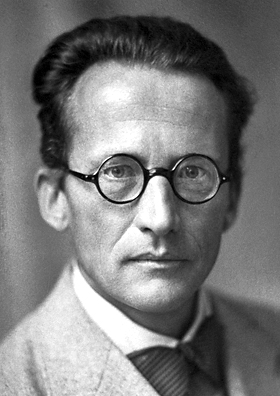
\includegraphics[width=\linewidth]{images/book4/schrodinger-1933.jpg}\par
{\footnotesize Schrödinger em 1933.}
\end{minipage}
\end{history}

\section{Exercícios}

\begin{exercise}[$\star$]\label{exo:b3:quantum-model-systems:1}
Um elétron está confinado em uma caixa de comprimento (a) \qty{1.00}{nm}, (b)
\qty{0.50}{nm}. Calcule $E_1$ em joules e em elétron-volts, e o comprimento de
onda da transição $n = 1 \to 2$.
\end{exercise}

\begin{exercise}[$\star$]\label{exo:b3:quantum-model-systems:2}
Liste os cinco níveis mais baixos de uma partícula em uma caixa cúbica, em
unidades de $h^2/8mL^2$, com suas \omterm{def:b3:quantum-model-systems:degenerate}{degenerescências}.
\end{exercise}

\begin{exercise}[$\star$]\label{exo:b3:quantum-model-systems:3}
Calcule os \omterm{def:b3:quantum-model-systems:commutator}{comutadores} $[\hat x^2,\hat p]$ e $[\hat p^2,\hat x]$ fazendo-os
agir sobre uma função $f(x)$.
\end{exercise}

\begin{exercise}[$\star$]\label{exo:b3:quantum-model-systems:4}
% ledger: diat:HCl.Be
Com $B = \qty{10.593}{cm^{-1}}$ para \ce{H^{35}Cl}, dê as energias (em
\unit{cm^{-1}}) e as \omterm{def:b3:quantum-model-systems:degenerate}{degenerescências} dos níveis $J = 0$ a 3, e o momento de
inércia da molécula.
\end{exercise}

\begin{exercise}[$\star\star$]\label{exo:b3:quantum-model-systems:5}
Para o estado $\psi_n$ de uma \omterm{def:b3:quantum-model-systems:box}{partícula na caixa}, calcule $\langle x\rangle$ e
$\langle x^2\rangle$. Avalie $\langle x^2\rangle$ para $n = 1$ e compare com
o valor clássico $L^2/3$ de uma partícula com igual probabilidade de estar em qualquer ponto.
\end{exercise}

\begin{exercise}[$\star\star$]\label{exo:b3:quantum-model-systems:6}
% ledger: diat:H2.we, diat:D2.we
Calcule as \omterm{def:b3:quantum-model-systems:oscillator}{energias do ponto zero} harmônicas de \ce{H2} e \ce{D2} em
\unit{kJ/mol} a partir de $\tilde\omega_e = \qty{4401.2}{cm^{-1}}$ e
\qty{3115.5}{cm^{-1}}, e sua diferença. Que razão de números de onda você
espera a partir das \omterm{def:b3:quantum-model-systems:oscillator}{massas reduzidas}, e quão próxima dela está a medida?
\end{exercise}

\begin{exercise}[$\star\star$]\label{exo:b3:quantum-model-systems:7}
A função $\phi = Nx(L - x)$ é um palpite grosseiro para o estado fundamental
da caixa. Normalize-a e depois calcule sua sobreposição $\langle\psi_1|\phi\rangle$
com o verdadeiro estado fundamental.
\end{exercise}

\begin{exercise}[$\star\star$]\label{exo:b3:quantum-model-systems:8}
Mostre que $\hat p = -\iu\hbar\,\dd/\dd x$ é \omterm{def:b3:quantum-model-systems:hermitian}{hermitiano} para funções que se
anulam nas extremidades de um intervalo, e que $\hat x\hat p$ não é.
\end{exercise}

\begin{exercise}[$\star\star$]\label{exo:b3:quantum-model-systems:9}
Modele o hexa-1,3,5-trieno como seis elétrons $\pi$ em uma caixa de comprimento $6l$, $l =
\qty{139.7}{pm}$ (cinco ligações e meia ligação em cada extremidade). Preveja o
comprimento de onda de sua primeira absorção. A molécula é colorida?
\end{exercise}

\begin{exercise}[$\star\star\star$]\label{exo:b3:quantum-model-systems:10}
Para a barreira-modelo da figura ($V_0 = \qty{0.40}{eV}$, $a = \qty{50}{pm}$)
em $E = V_0/2$, calcule $\kappa$ para um próton e para um dêuteron e, com a
fórmula da barreira espessa, a razão $T_H/T_D$. Compare com a razão exata, 58.
\end{exercise}

\begin{exercise}[$\star\star\star$]\label{exo:b3:quantum-model-systems:11}
Trate os seis elétrons $\pi$ do benzeno como partículas em um anel de raio
\qty{139.7}{pm} (a distância C--C é igual ao raio de um hexágono regular).
Preencha os níveis e depois calcule o comprimento de onda da transição do
nível preenchido mais alto para o nível vazio mais baixo.
\end{exercise}

\begin{exercise}[$\star\star\star$]\label{exo:b3:quantum-model-systems:12}
Para o estado $1s$ do hidrogênio, $\psi = (\pi a^3)^{-1/2}\eu^{-r/a}$. Calcule os
\omterm{def:b3:quantum-model-systems:hermitian}{valores esperados} $\langle r\rangle$ e $\langle V\rangle$, e verifique que
$\langle V\rangle = 2E_1$. (Use $\int_0^\infty r^n\eu^{-\beta r}\dd r =
n!/\beta^{n+1}$.)
\end{exercise}

\section{Problema: Qual é o comprimento de um corante?}

\begin{problem}[{Problema de fim de semana --- o modelo do elétron livre de três
corantes de cianina: por que a cadeia sem extensão falha, quais transições são
permitidas, as escalas de energia de uma molécula e o comprimento de caixa que se ajusta}]
\label{pb:b3:quantum-model-systems:1}
% ledger: uvvis:cyanine, uvvis:carbocyanine, uvvis:dicarbocyanine, geo:C6H6.rCC, diat:HCl.we, diat:HCl.Be
Três corantes de cianina simétricos absorvem em 524, 603 e 711 nm em etanol;
suas cadeias conjugadas, entre os dois nitrogênios e incluindo-os, têm $j = 5$, 7
e 9 átomos. Tome cada ligação igual a $l = \qty{139.7}{pm}$, $m_e =
\qty{9.109e-31}{kg}$, $h = \qty{6.626e-34}{J.s}$, $c = \qty{2.998e8}{m/s}$,
$k = \qty{1.381e-23}{J/K}$, $\qty{1}{eV} = \qty{1.602e-19}{J}$.

\medskip\noindent\textbf{Parte I --- A cadeia sem extensão.}
\begin{enumerate}
  \item Explique por que uma cadeia de $j$ átomos carrega $N = j + 1$ elétrons $\pi$, e
        dê $N$ para cada corante.
  \item Quais níveis da caixa são o preenchido mais alto e o vazio mais baixo
        para o primeiro corante?
  \item Mostre que a primeira absorção está em $\lambda = 8mcL^2/h(N+1)$.
  \item Dê o comprimento sem extensão $L_0 = (j - 1)l$ de cada cadeia.
  \item Calcule $\lambda$ para cada corante com $L = L_0$.
  \item Compare com os valores medidos. Em que sentido o modelo erra, e o
        que isso diz sobre $L$?
\end{enumerate}

\medskip\noindent\textbf{Parte II --- Quais transições são permitidas.}
A intensidade de uma transição $n \to n'$ é proporcional a $|\langle
\psi_n|x - L/2|\psi_{n'}\rangle|^2$.
\begin{enumerate}[resume]
  \item Mostre que $\psi_n$ é simétrica em relação ao centro da caixa para $n$
        ímpar e antissimétrica para $n$ par.
  \item Deduza que a integral se anula quando $n + n'$ é par.
  \item A transição HOMO $\to$ LUMO de cada corante é permitida?
  \item Para o segundo corante, a transição do HOMO para o nível acima do
        LUMO é permitida? E a do nível abaixo do HOMO para o LUMO?
  \item No modelo, em que comprimento de onda (como fração do primeiro)
        estaria a próxima transição permitida a partir do HOMO?
  \item Por que uma regra como essa, deduzida apenas da simetria, sobrevive
        à grosseria do modelo?
\end{enumerate}

\medskip\noindent\textbf{Parte III --- As escalas de energia de uma molécula.}
\begin{enumerate}[resume]
  \item Converta a absorção do segundo corante em uma energia em eV.
  \item A vibração de \ce{HCl} tem $\tilde\omega_e = \qty{2991}{cm^{-1}}$:
        converta seu quantum em eV.
  \item A rotação de \ce{HCl} tem $B = \qty{10.59}{cm^{-1}}$: converta o
        intervalo entre $J = 0$ e $J = 1$ em meV.
  \item Calcule $kT$ em meV a \qty{298}{K}.
  \item Quais tipos de excitação estão povoados à temperatura ambiente?
  \item Em quais regiões do espectro se observam as transições eletrônicas,
        vibracionais e rotacionais?
\end{enumerate}

\medskip\noindent\textbf{Parte IV --- A caixa que se ajusta.}
\begin{enumerate}[resume]
  \item A partir dos 603 nm medidos, calcule o comprimento $L$ que a caixa do
        segundo corante deve ter.
  \item Escrevendo $L = L_0 + 2\delta$, deduza $\delta$.
  \item Com esse $\delta$, preveja $\lambda$ para o primeiro corante; dê o
        erro relativo.
  \item Mesma pergunta para o terceiro corante.
  \item Interprete $\delta$: para onde vão os elétrons $\pi$ além dos
        nitrogênios?
  \item Expresse $\delta$ em comprimentos de ligação e enuncie o resultado do
        problema: a extensão efetiva da caixa em cada extremidade.
\end{enumerate}
\end{problem}
